\documentclass{leaflet}
\usepackage{palatino}
\usepackage{url}
\title{Milkymist\texttrademark~One\\Video Synthesizer}
\date{}
\begin{document}
\maketitle
\thispagestyle{empty}
\pagestyle{empty} 
\textit{Congratulations on your purchase of a Milkymist One video synthesizer. We hope you will make good use of this powerful tool to create stunning and artistic visual effects.}

\section{Quick start guide}
Just follow those four super-easy steps to get started with Milkymist One generated visuals in no time.

\subsection{Connect the power supply}
Use the provided 5V supply adapter to power the Milkymist One. \textbf{Do not use the 12V adapter} which is for the camera.

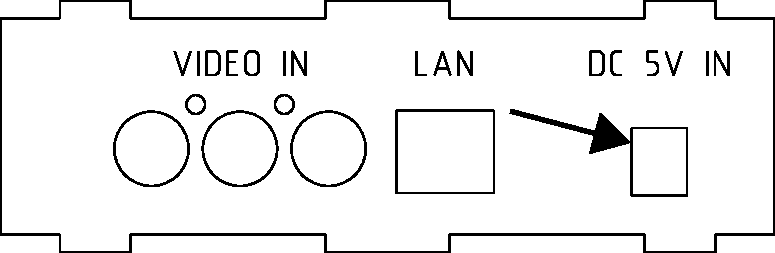
\includegraphics[width=\textwidth]{power.pdf}

\subsection{Connect the video projector}
Connect a VGA video projector (or a simple screen) to the video output of the Milkymist One.

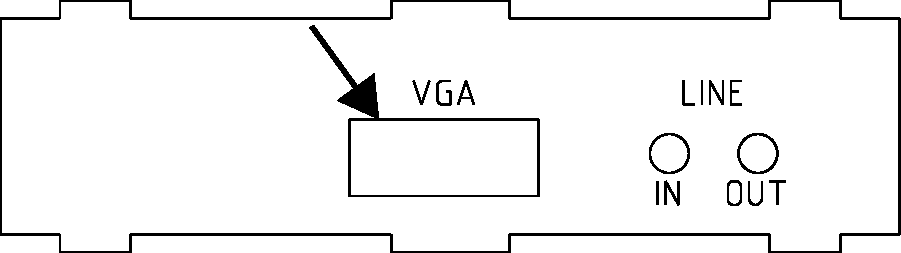
\includegraphics[width=\textwidth]{vga.pdf}

\subsection{Connect the camera}
Using the provided cable, connect the RCA jack of the camera to the \textbf{green} RCA jack of the Milkymist One. \textit{The other two RCA jacks are used for S-Video and component (RGB) video sources, and not for audio.}

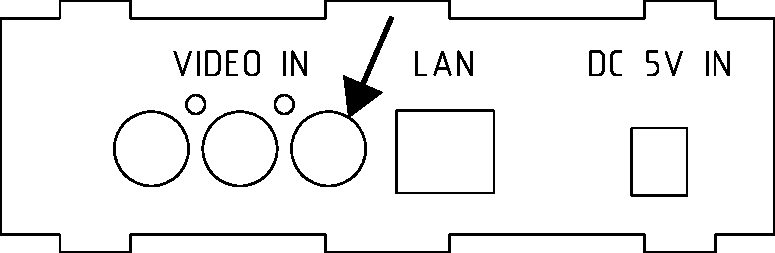
\includegraphics[width=\textwidth]{videoin.pdf}

Use the provided 12V supply adapter to power the camera. \textbf{Do not use the 5V adapter} which is for the Milkymist One.

For the best visual results, use a black background and proper lighting.

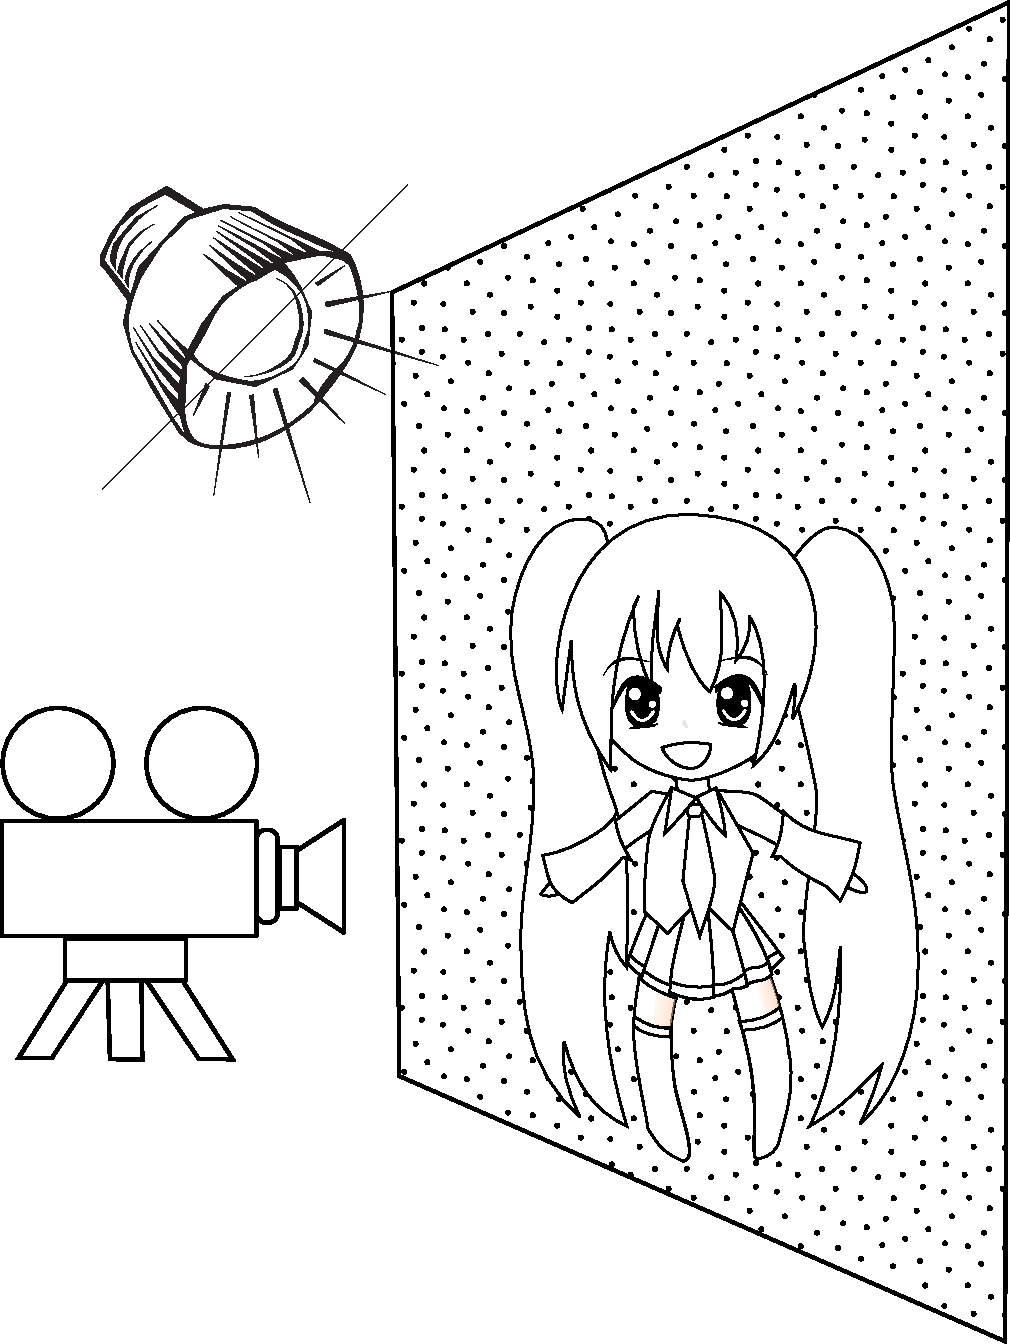
\includegraphics[width=80mm]{camsetup.pdf}

\subsection{Enjoy}
Press the middle pushbutton on the Milkymist One to start.

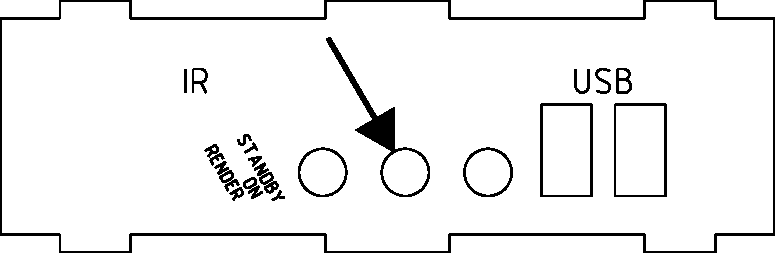
\includegraphics[width=\textwidth]{midpb.pdf}

After a dozen seconds, the effects start appearing on the projector.

Some effects use the image captured from the camera, while some others do not and are purely generative. Similarly, some effects are reactive to sound, which can be picked up from the internal microphone or fed using the line input minijack. Have fun!

When you want to turn off the Milkymist One, hold the middle pushbutton for a few seconds.

\section{To go further...}
You will probably want to customize the visual experience generated by the synthesizer.

Connect a USB keyboard (provided) and a USB mouse (not provided) to the Milkymist One. Press the Enter key to stop generating visual effects and enter the configuration interface.

Like a computer, the configuration interface uses a windowed system with mouse and keyboard interaction. From there, you can define what visual effects are selected when in performance mode, associate them to key presses on the USB keyboard, map them to the keys of a MIDI keyboard, and more. You can even write your own snippets of code (called ``patches'') using the Flickernoise Patching (FNP) programming language to create totally new visual experiences. Find out more at \url{www.milkymist.org}.

If you do not have a suitable USB mouse available, you can use the keyboard to move the pointer and click. Just hold the Meta key while you use the arrows keys to move and the Enter key to click.

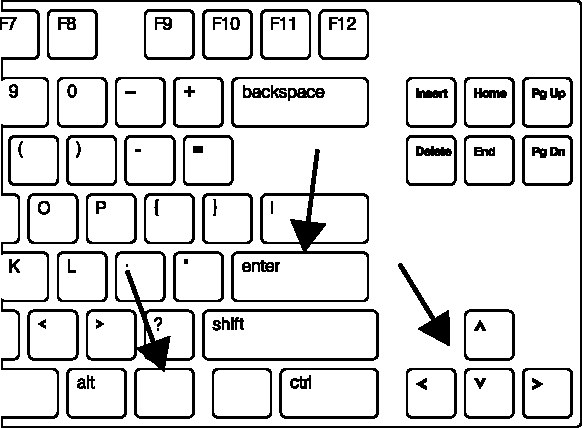
\includegraphics[width=\textwidth]{keyboard.pdf}

\section{Software updates}
It's easy to keep your Milkymist One up to date with the latest software and the latest visual effects (patches). Use the Ethernet port to connect it to the Internet. By default, the device will use DHCP to set up the connection, which should automatically work fine on most networks. If your network does not use DHCP, use the configuration interface to set up the connection manually.

To proceed with the update, simply hold the left pushbutton for a few seconds. The update dialog will pop up as the device downloads the latest software and patches.

Once this is done, turn off and on again the device to use the new software.

\section{Contents}
The Milkymist One has everything on board for you to create the most psychedelic interactive visual performances:
\begin{itemize}
\item Analogue video input with low latency -- step inside the visuals and dance!
\item Two DMX512 ports -- program a light ambiance in harmony with the visual effects.
\item MIDI IN and MIDI OUT ports -- communicate with MIDI controllers and keyboards, or even Arduino boards (\url{www.arduino.cc}).
\item Audio with integrated microphone and line input -- synchronize easily to the beat!
\item Ethernet -- go online to grab new visual creations, set up a ``tweet wall'' in a few clicks, and more!
\item Infrared receiver for RC5 remote controls
\item High resolution VGA output
\item Two USB host connectors
\end{itemize}

Along with a Milkymist One video synthesizer, your box contains the following accessories:
\begin{itemize}
\item a CVBS mini-camera
\item a silicone USB keyboard
\item an RCA video cable
\item a minijack-minijack and a minijack-RCA audio cables
\item an Ethernet cable
\item a 5V power supply adapter for the Milkymist One
\item a 12V power supply adapter for the camera
\item development and repair tools:
\begin{itemize}
\item a programming adapter (JTAG/serial)
\item a USB cable for the programming adapter
\end{itemize}
\end{itemize}

\section{Warranty and return policy}
The Milkymist One is manufactured by Sharism at Work Ltd. (\url{www.sharism.cc}). The devices are fully factory tested, and are guaranteed against manufacturing defects for a period of 3 years after the date of initial purchase. This does not include malfunction due to misuse of the device, such as application of inappropriate voltages to the device's connectors or improperly designed or executed modifications. In particular, you are the sole responsible for damage caused by a power supply adapter other than provided, or by mistaking the video camera and the Milkymist One power supplies.

If you believe your device suffers from a manufacturing problem, e-mail sales@sharism.cc and we will find a solution and/or replace the faulty product.

\section{Open source hardware and software}
The people who brought you the Milkymist One are strong believers in open source. All the hardware and software designs we have developed to build this device, including the full Verilog HDL sources of the system-on-chip design, are published under free and open source licenses such as GNU GPL and Creative Commons BY-SA. Under the terms of those licenses, you are welcome to copy our designs, improve them, contribute your changes back, and re-use them in your own open source projects. Find out more at \url{www.milkymist.org}.

Thank you again for your purchase of a Milkymist One video synthesizer. Feel free to send us your questions, feedback, bug reports and even links to pictures or videos of your performances to devel@lists.milkymist.org. Alternatively, you can come in our IRC channel \#milkymist on Freenode. We hope to hear from you soon!

\textit{This leaflet is published under the Creative Commons Attribution-ShareAlike 3.0 Unported license. Milkymist is a trademark of S\'ebastien Bourdeauducq.}

\begin{center}
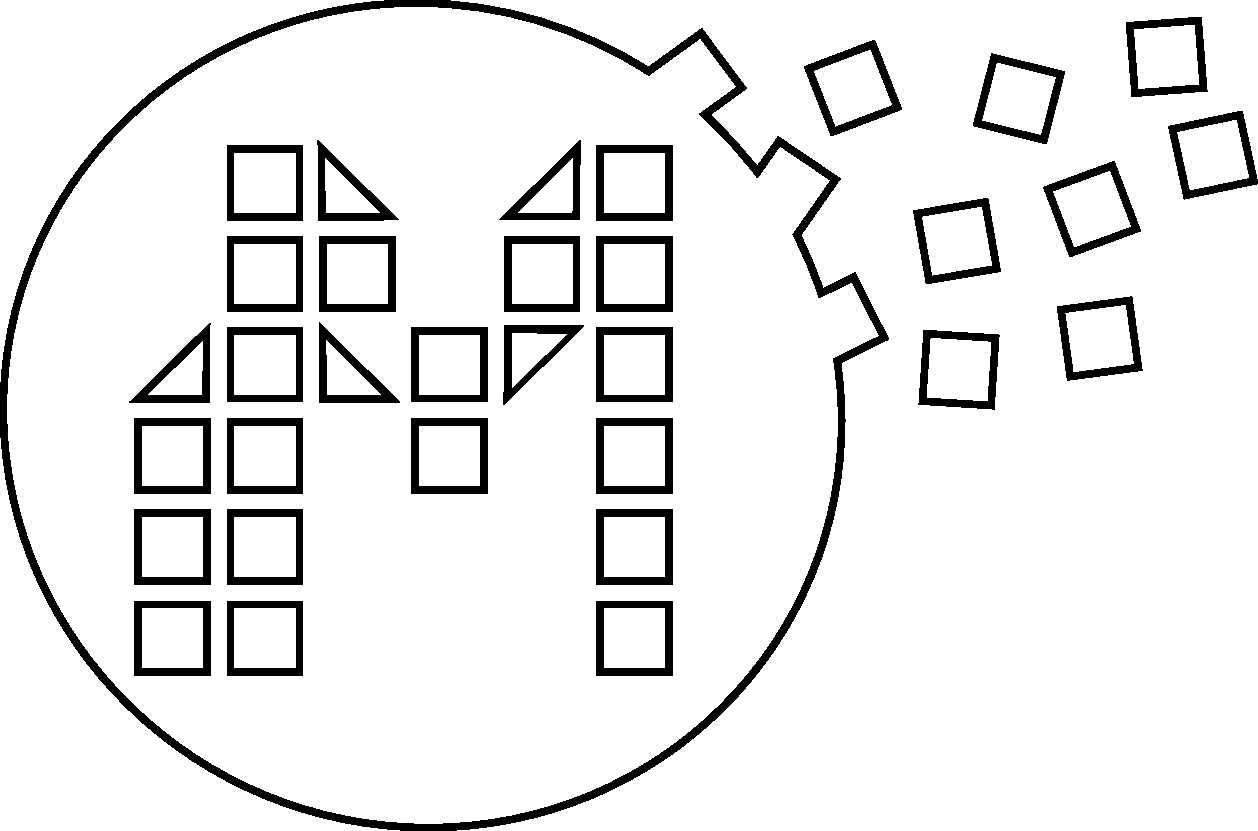
\includegraphics[width=40mm]{logo.pdf} \\
\textbf{www.milkymist.org}
\end{center}

\end{document}
